\chapter{Producing Our Food}\label{ch:g6:producing-our-food}

Nothing on your breakfast table was found in the wild. The
bread's wheat was bred and farmed; the \omterm{def:g2:animals-grow-up:born}{milk} came from herds
tended for it; the yogurt was \emph{made} from that \omterm{def:g2:animals-grow-up:born}{milk} by
billions of living workers too small to see. Humans feed
themselves by managing \omterm{def:g6:exploring-our-environment:components}{living things} --- growing them,
raising them, and putting some of the smallest to work. This
chapter tours the food workshop.

\section{Growing and raising}

\begin{definition}[Crops and livestock]\label{def:g6:producing-our-food:farming}
Human food production manages \omterm{def:g6:exploring-our-environment:components}{living things} at two floors of
the matter cycle:
\begin{itemize}
  \item \emph{crop growing}\index{crop}: managing \omterm{def:g5:food-webs:roles}{producers}
        --- wheat, potatoes, vegetables, \omterm{prop:g3:flowers-fruits-seeds:transform}{fruit} --- for their
        \omterm{def:g6:plants-are-producers:matter}{organic matter}
        (\cref{prop:g6:plants-are-producers:produce});
  \item \emph{livestock raising}\index{livestock}: managing
        \omterm{def:g5:food-webs:roles}{consumers} --- cattle, sheep, pigs, hens --- for
        their \omterm{def:g6:matter-from-food:production}{production of matter}
        (\cref{def:g6:matter-from-food:production}): \omterm{def:g2:animals-grow-up:born}{milk},
        meat, \omterm{def:g2:animals-grow-up:born}{eggs}, wool.
\end{itemize}
Farmers manage the \omterm{def:g6:exploring-our-environment:conditions}{conditions} this book keeps meeting: \omterm{def:g6:decomposers-and-soil:soil}{soil}
minerals for the crops (\cref{rem:g4:what-plants-need:soil}),
feed for the \omterm{def:g1:animals-around-us:animal}{animals} --- the whole ledger of
\cref{pb:g6:matter-from-food:1}, run on purpose.
\end{definition}

\begin{example}[What a wheat field is]\label{ex:g6:producing-our-food:wheat}
A wheat field is a managed \omterm{def:g6:exploring-our-environment:components}{environment}
(\cref{prop:g5:people-and-nature:managed}) tuned for one
\omterm{def:g5:food-webs:roles}{producer}: \omterm{def:g6:decomposers-and-soil:soil}{soil} restocked and loosened for its \omterm{def:g1:plants-around-us:parts}{roots},
sowing timed to \cref{prop:g2:from-seed-to-plant:needs}'s
warmth, weeds --- rival colonists of
\cref{ch:g6:how-plants-spread} --- kept out. The harvest is
the \omterm{def:g1:plants-around-us:plant}{plant}'s \omterm{def:g2:from-seed-to-plant:seed}{seed} store: grain, the packed lunches of a
million never-to-be-sown wheat \omterm{def:g1:plants-around-us:plant}{plants}, diverted to bakeries.
\end{example}

\begin{remark}[Every food is a life-cycle stage]\label{rem:g6:producing-our-food:stage}
Read any food biologically and it is some organism's organ
or stage: grain and beans are \omterm{def:g2:from-seed-to-plant:seed}{seed} stores; potatoes, \omterm{ex:g4:plants-without-seeds:bulbtuber}{tubers};
apples, \omterm{prop:g3:flowers-fruits-seeds:transform}{fruits} built to be eaten
(\cref{exo:g6:how-plants-spread:12}); \omterm{def:g2:animals-grow-up:born}{milk} is mammal
mother-care (\cref{def:g2:animals-grow-up:born}); an \omterm{def:g2:animals-grow-up:born}{egg} is
a packed nursery. Food production is the art of managing
\omterm{def:g2:born-grow-die:cycle}{life cycles} so their provisions arrive on our tables.
\end{remark}

\section{The invisible workforce: food made by microbes}

\begin{definition}[Fermentation]\label{def:g6:producing-our-food:fermentation}
Some foods are made by putting \omterm{def:g6:exploring-our-environment:components}{living things} too small to
see --- \emph{microbes}\index{microbe (food)} --- to work on
a raw material. Their feeding transforms it: the
transformation is called
\emph{fermentation}\index{fermentation}, and humans have run
it for thousands of years, since long before anyone knew
the workers existed.
\end{definition}

\begin{example}[Bread rises]\label{ex:g6:producing-our-food:bread}
Bread's raw dough is flour and water --- plus
\emph{yeast}\index{yeast}, a single-celled \omterm{def:g6:decomposers-and-soil:decomposers}{fungus}
(\cref{rem:g5:first-look-at-cells:onecelled} met such
lives). The \omterm{ex:g6:producing-our-food:bread}{yeast} feeds on the flour's sugars and releases
a gas; the gas's bubbles, trapped in the stretchy dough,
puff it up --- the baker calls it rising. The oven's heat
then ends the workers' shift and sets their work: the
crumb's holes are the \omterm{ex:g6:producing-our-food:bread}{yeast}'s signature.
\end{example}

\begin{omfigure}
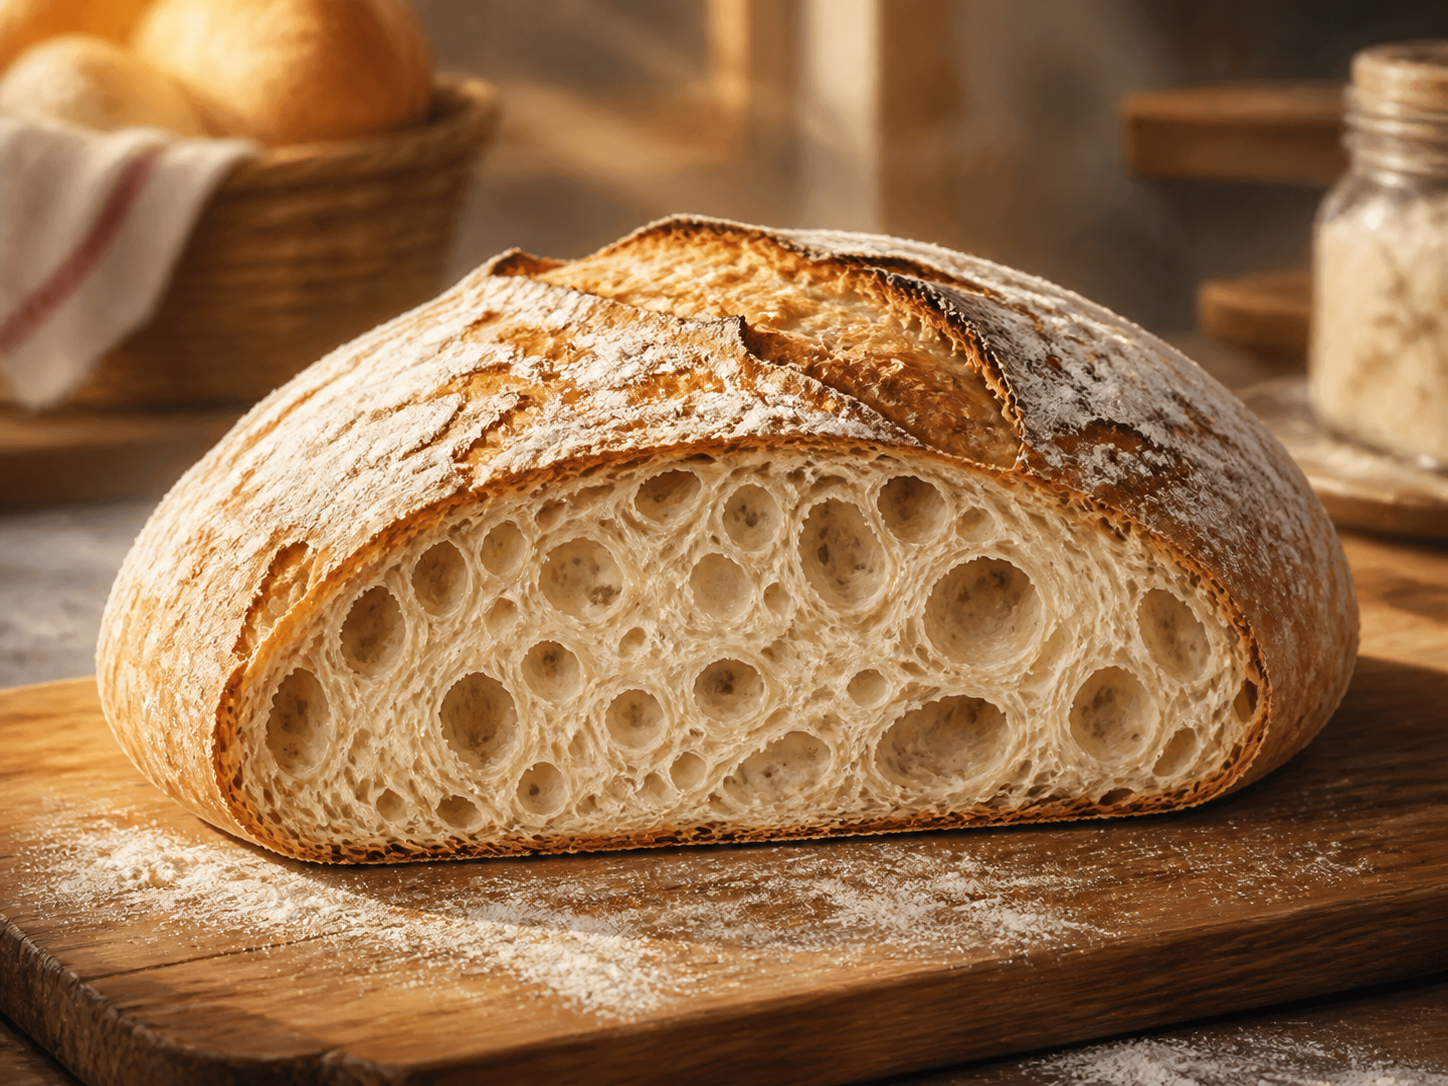
\includegraphics[width=0.58\linewidth]{images/book1/ai/g6-food-bread.png}

{\small The workforce's signature, baked in place: every hole
in the crumb is a bubble the \omterm{ex:g6:producing-our-food:bread}{yeast} blew.}
\end{omfigure}

\begin{example}[Milk becomes yogurt and cheese]\label{ex:g6:producing-our-food:yogurt}
Warm \omterm{def:g2:animals-grow-up:born}{milk} seeded with the right \omterm{def:g6:producing-our-food:fermentation}{microbes} thickens overnight
into yogurt: the workers feed on the \omterm{def:g2:animals-grow-up:born}{milk}'s sugar and
release an acid, and the acid sets the \omterm{def:g2:animals-grow-up:born}{milk} --- the fresh
tang \emph{is} the acid. Cheese starts similarly, then goes
further: curds pressed, salted and ripened for months, the
\omterm{def:g6:producing-our-food:fermentation}{microbes} working on through the ripening --- a cheese's
holes, rind and power of smell are their long shift's log.
\end{example}

\begin{remark}[Helpful and harmful microbes]\label{rem:g6:producing-our-food:goodbad}
The \omterm{def:g1:healthy-habits:germs}{germs} of \cref{def:g1:healthy-habits:germs} taught
caution about \omterm{def:g6:producing-our-food:fermentation}{microbes}; this chapter adds the other half:
\emph{chosen} \omterm{def:g6:producing-our-food:fermentation}{microbes}, working in \emph{controlled}
\omterm{def:g6:exploring-our-environment:conditions}{conditions}, are among our oldest employees --- in bread,
yogurt, cheese, and the vinegar barrel. The craft is always
the same: welcome the chosen workers, and keep \omterm{def:g6:exploring-our-environment:conditions}{conditions}
that suit them and not the spoilers. Salting, cooling,
drying and cooking are all ways of refusing \omterm{def:g6:exploring-our-environment:conditions}{conditions} to
unwanted \omterm{def:g6:producing-our-food:fermentation}{microbes} (\cref{prop:g6:decomposers-and-soil:speed}
works on a ham exactly as on a \omterm{def:g1:plants-around-us:parts}{leaf} pile).
\end{remark}

\section{From field to table, honestly}

\begin{proposition}[The costs on the table]\label{prop:g6:producing-our-food:costs}
Every plate is an output of managed land and \omterm{def:g6:exploring-our-environment:components}{living things},
and carries their arithmetic:
\begin{itemize}
  \item \omterm{def:g1:plants-around-us:plant}{plant} foods arrive one floor from the \omterm{def:g6:exploring-our-environment:conditions}{light}; \omterm{def:g1:animals-around-us:animal}{animal}
        foods route through a \omterm{def:g5:food-webs:roles}{consumer} first and pay
        \cref{prop:g6:matter-from-food:losses}'s toll
        (\cref{exo:g6:matter-from-food:12});
  \item lasting production must keep
        \cref{prop:g5:people-and-nature:lasting}'s three
        rules --- feed the \omterm{def:g6:decomposers-and-soil:soil}{soil}, keep the helpers, take no
        faster than renewal;
  \item and waste undoes it all: food thrown away spent its
        land, water and work for no one.
\end{itemize}
\end{proposition}
\admitted

\begin{method}[Reading a food's story]\label{met:g6:producing-our-food:read}
For any food in the kitchen:
\begin{enumerate}
  \item name the organism and the organ or stage it is
        (\cref{rem:g6:producing-our-food:stage});
  \item place it on the cycle: \omterm{def:g5:food-webs:roles}{producer}'s matter, \omterm{def:g5:food-webs:roles}{consumer}'s
        product, or microbe-made?
  \item if microbe-made, name the raw material and what the
        workers changed;
  \item trace it to its \omterm{def:g1:plants-around-us:parts}{leaf}
        (\cref{met:g6:plants-are-producers:trace}) --- the
        trail still always ends in the \omterm{def:g6:exploring-our-environment:conditions}{light}.
\end{enumerate}
\end{method}

\begin{example}[The method at breakfast]\label{ex:g6:producing-our-food:breakfast}
Yogurt, by the method: (1) \omterm{def:g2:animals-grow-up:born}{milk} --- a cow's mother-care
product --- transformed; (2) \omterm{def:g5:food-webs:roles}{consumer}'s product,
microbe-finished; (3) raw material \omterm{def:g2:animals-grow-up:born}{milk}, workers soured and
set it; (4) \omterm{def:g2:animals-grow-up:born}{milk} from the cow, cow from grass, grass from
\omterm{def:g6:exploring-our-environment:conditions}{light}. Three organisms and a workforce of billions, in one
small pot.
\end{example}

\section{Exercises}

\begin{exercise}[$\star$]\label{exo:g6:producing-our-food:1}
Define \omterm{def:g6:producing-our-food:farming}{crop growing} and \omterm{def:g6:producing-our-food:farming}{livestock raising}, naming the floor
of the matter cycle each manages.
\end{exercise}

\begin{exercise}[$\star$]\label{exo:g6:producing-our-food:2}
For each food, name the organism and the organ or stage:
grain, potato, apple, \omterm{def:g2:animals-grow-up:born}{milk}, \omterm{def:g2:animals-grow-up:born}{egg}.
\end{exercise}

\begin{exercise}[$\star$]\label{exo:g6:producing-our-food:3}
What is \omterm{def:g6:producing-our-food:fermentation}{fermentation}? Name two fermented foods and their
raw materials.
\end{exercise}

\begin{exercise}[$\star$]\label{exo:g6:producing-our-food:4}
Tell why bread rises: the worker, its food, what it
releases, and what the oven does.
\end{exercise}

\begin{exercise}[$\star$]\label{exo:g6:producing-our-food:5}
What sets \omterm{def:g2:animals-grow-up:born}{milk} into yogurt, and where does the tang come
from?
\end{exercise}

\begin{exercise}[$\star$]\label{exo:g6:producing-our-food:6}
Give three ways of refusing \omterm{def:g6:exploring-our-environment:conditions}{conditions} to unwanted
\omterm{def:g6:producing-our-food:fermentation}{microbes}, from \cref{rem:g6:producing-our-food:goodbad}.
\end{exercise}

\begin{exercise}[$\star\star$]\label{exo:g6:producing-our-food:7}
A wheat field manages every need of
\cref{prop:g4:what-plants-need:needs} on purpose. Match
each need to the farmer's action of
\cref{ex:g6:producing-our-food:wheat}.
\end{exercise}

\begin{exercise}[$\star\star$]\label{exo:g6:producing-our-food:8}
Run \cref{met:g6:producing-our-food:read} on cheese, step
by step.
\end{exercise}

\begin{exercise}[$\star\star$]\label{exo:g6:producing-our-food:9}
Why does refrigeration keep food --- and why does the same
cold slow a compost heap? One principle, two kitchens:
name it.
\end{exercise}

\begin{exercise}[$\star\star$]\label{exo:g6:producing-our-food:10}
Reconcile \cref{def:g1:healthy-habits:germs} with this
chapter: how can \omterm{def:g6:producing-our-food:fermentation}{microbes} be both the hand-washing enemy
and the yogurt workforce?
\end{exercise}

\begin{exercise}[$\star\star$]\label{exo:g6:producing-our-food:11}
Using \cref{prop:g6:producing-our-food:costs}, explain why
a thrown-away ham sandwich wastes more than the same
weight of thrown-away bread.
\end{exercise}

\begin{exercise}[$\star\star\star$]\label{exo:g6:producing-our-food:12}
For thousands of years, bakers and brewers ran
\omterm{def:g6:producing-our-food:fermentation}{fermentation} without knowing \omterm{def:g6:producing-our-food:fermentation}{microbes} existed. What did
they actually manage, in
\cref{prop:g6:exploring-our-environment:decide}'s terms
--- and why did their recipes work anyway?
\end{exercise}

\section{Problem: The Class Bakery}

\begin{problem}[{Weekend problem --- one batch of bread,
followed from seed to slice}]\label{pb:g6:producing-our-food:1}
For the school fair, the class bakes bread from scratch ---
and keeps its \omterm{def:g1:living-or-not:living}{biology} notebook open from the wheat field
visit in July to the loaves in November.

\medskip\noindent\textbf{Part I --- The field (July).}
\begin{enumerate}
  \item The farmer shows the ripe wheat: ``the harvest is
        the \omterm{def:g1:plants-around-us:plant}{plant}'s packed lunches.'' Unpack the phrase
        with \cref{def:g2:from-seed-to-plant:seed} --- what
        is each grain, and for whom was it packed?
  \item In whose \omterm{def:g1:plants-around-us:parts}{leaves}, and with what inputs, was the
        grain's \omterm{def:g6:plants-are-producers:matter}{organic matter} manufactured?
  \item The farmer sows only part of the harvest next
        autumn and sells the rest. Name the two fates of a
        wheat grain, in life-cycle terms.
  \item The field's \omterm{def:g6:decomposers-and-soil:soil}{soil} gets manure after harvest. Which
        return rule is this, and which of the \omterm{def:g1:plants-around-us:plant}{plant}'s five
        needs does it serve?
\end{enumerate}

\medskip\noindent\textbf{Part II --- The bakery (November).}
\begin{enumerate}[resume]
  \item The class mixes flour, water, salt and \omterm{ex:g6:producing-our-food:bread}{yeast}, and
        sets the dough in a warm corner. Why warm? Answer
        for the \omterm{ex:g6:producing-our-food:bread}{yeast} as for any living worker
        (\cref{prop:g6:decomposers-and-soil:speed} has the
        pattern).
  \item An hour later the dough has doubled. Explain the
        rise: what did the \omterm{ex:g6:producing-our-food:bread}{yeast} feed on, what did it
        release, and what trapped it?
  \item One team's dough, forgotten by a drafty cold
        window, barely rises. Diagnose --- and say which
        fair-test comparison the two teams have
        accidentally run.
  \item In the oven the loaves stop rising and set. What
        has the heat done to the workforce, and what
        remains as its signature in the crumb?
\end{enumerate}

\medskip\noindent\textbf{Part III --- The accounting.}
\begin{enumerate}[resume]
  \item Trace the finished slice to the \omterm{def:g6:exploring-our-environment:conditions}{light}, link by
        link.
  \item The fair also sells butter and ham sandwiches.
        Rank slice, butter and ham by the floors their
        matter routed through, and state which paid the
        biggest toll of
        \cref{prop:g6:matter-from-food:losses}.
  \item Unsold dough is composted, not binned. Follow its
        \omterm{def:g6:plants-are-producers:matter}{organic matter} one turn further around the cycle
        --- who takes it, and toward what?
  \item Close the notebook with one sentence containing:
        \omterm{def:g5:food-webs:roles}{producer}, \omterm{def:g5:food-webs:roles}{consumer} (if any), microbe workforce,
        and \omterm{def:g6:exploring-our-environment:conditions}{light}.
\end{enumerate}
\end{problem}
